\subsection[Scenariusz - Pharming (Jakub Wyka)]{Scenariusz - Pharming}
Założenia początkowe:
	-Raspberry Pi Zero z dostępem do internetu przez sieć wi-fi
	-Przewód usb – micro usb łączący Raspberry Pi Zero z komputerem ofiary
	- Raspberry Pi Zero połączone z serwerem sterującym
	- Pentester zalogowany w serwerze sterującym
Aktorzy:
	-Pentester
	- Serwer sterujący
	- testowany system
	-Raspberry Pi Zero
Opis testu:
Zatruwanie DNS to metoda ataku polegająca na zmianie rekordu w DNS, która fałszywie przypisuje nazwę domeny do adresu IP.  Zadaniem tego ataku jest przekierowanie użytkownika na inną stronę niż ta, którą faktycznie chciał otworzyć. Często witryna podszywająca się wygląda tak samo, przez co użytkownik nie jest świadomy ataku. Podszywanie to jest nazywane phishingiem. W ten sposób użytkownik logując się do serwisu dostarcza wrażliwe dane osobom przeprowadzającym atak. Połączenie DNS spoofingu z zaawansowanym phishingiem nazywane jest pharmingiem.

Przebieg:
Serwer sterujący służy do wydawania poleceń przez pentestera. Wybiera on, za pomocą którego z dostępnych urządzeń testujących ma zostać przeprowadzony test. Następnie wybiera rodzaj testu. W tym przypadku będzie to pharming. Serwer udostępni możliwość określenia konkretnych parametrów ataku. Dla tego typu ataku będzie to rekord DNS, który określi pod jaką domenę chcemy się podszyć oraz ip strony podszywającej. Serwer przesyła te dane do Raspberry Pi Zero, które na tej podstawie uruchamia skrypt, który jest odpowiedzialny za przeprowadzenie ataku. Do serwera odsyłany jest raport z wynikiem testu. 
\begin{figure}[H]
    \centering
    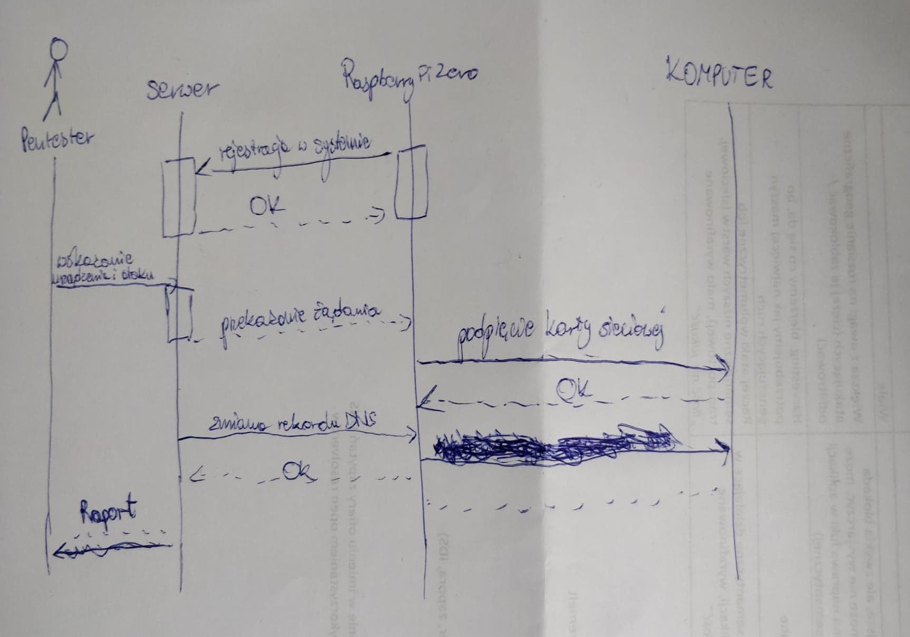
\includegraphics[width=\textwidth]{jw02}
    \caption{Pharming}
    \label{fig:pharming1}    
\end{figure}
\begin{figure}[H]
    \centering
    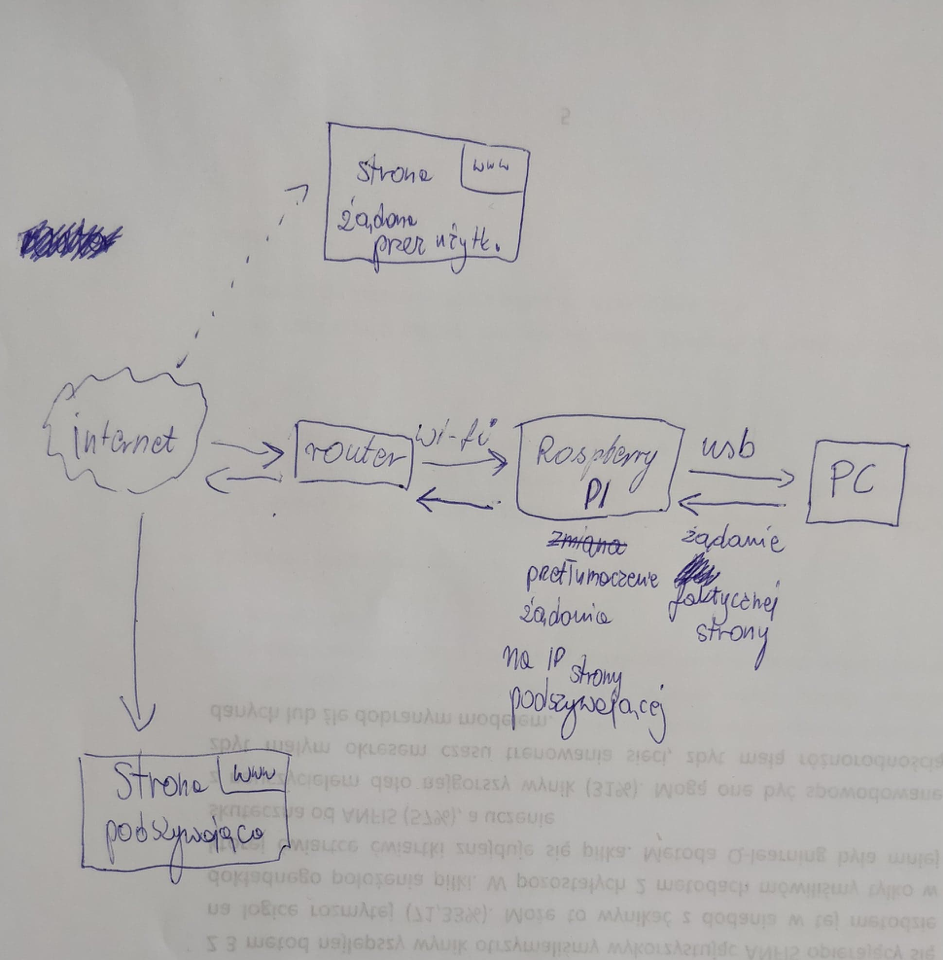
\includegraphics[width=\textwidth]{jw03}
    \caption{Pharming2}
    \label{fig:pharming2}    
\end{figure}